\chapter{La RMN du proton}\label{ch:g12:proton-nmr}

À l'hôpital, un patient est allongé dans l'anneau d'un appareil d'IRM, et
une image des tissus mous du corps apparaît à l'écran, construite à
partir des réponses des noyaux d'hydrogène de son eau et de ses graisses.
Au laboratoire de chimie, un petit tube de verre contenant quelques
milligrammes d'un composé descend dans l'alésage d'un aimant puissant,
et un spectre apparaît, construit de la même façon~: un aimant intense,
un signal radio, et des noyaux d'hydrogène qui y répondent. Dans le
spectromètre du chimiste, chaque \omterm{def:g9:inside-the-atom:nucleus}{noyau} d'hydrogène répond un peu
différemment selon ses voisins, et le spectre est une carte des \omterm{def:g7:atoms-and-molecules:atom}{atomes}
d'hydrogène de la \omterm{def:g7:atoms-and-molecules:molecule}{molécule}.

\begin{recall}
Un \omterm{def:g11:infrared:spectrum}{spectre infrarouge} montre quelles liaisons une \omterm{def:g7:atoms-and-molecules:molecule}{molécule} contient
(\cref{ch:g11:infrared}). \omterm{def:g11:functional-groups:functional-group}{Groupes caractéristiques}, familles et \omterm{def:g11:organic-skeletons:isomer}{isomères}
(\cref{ch:g11:functional-groups}, \cref{ch:g11:organic-skeletons}).
\end{recall}

\begin{omfigure}
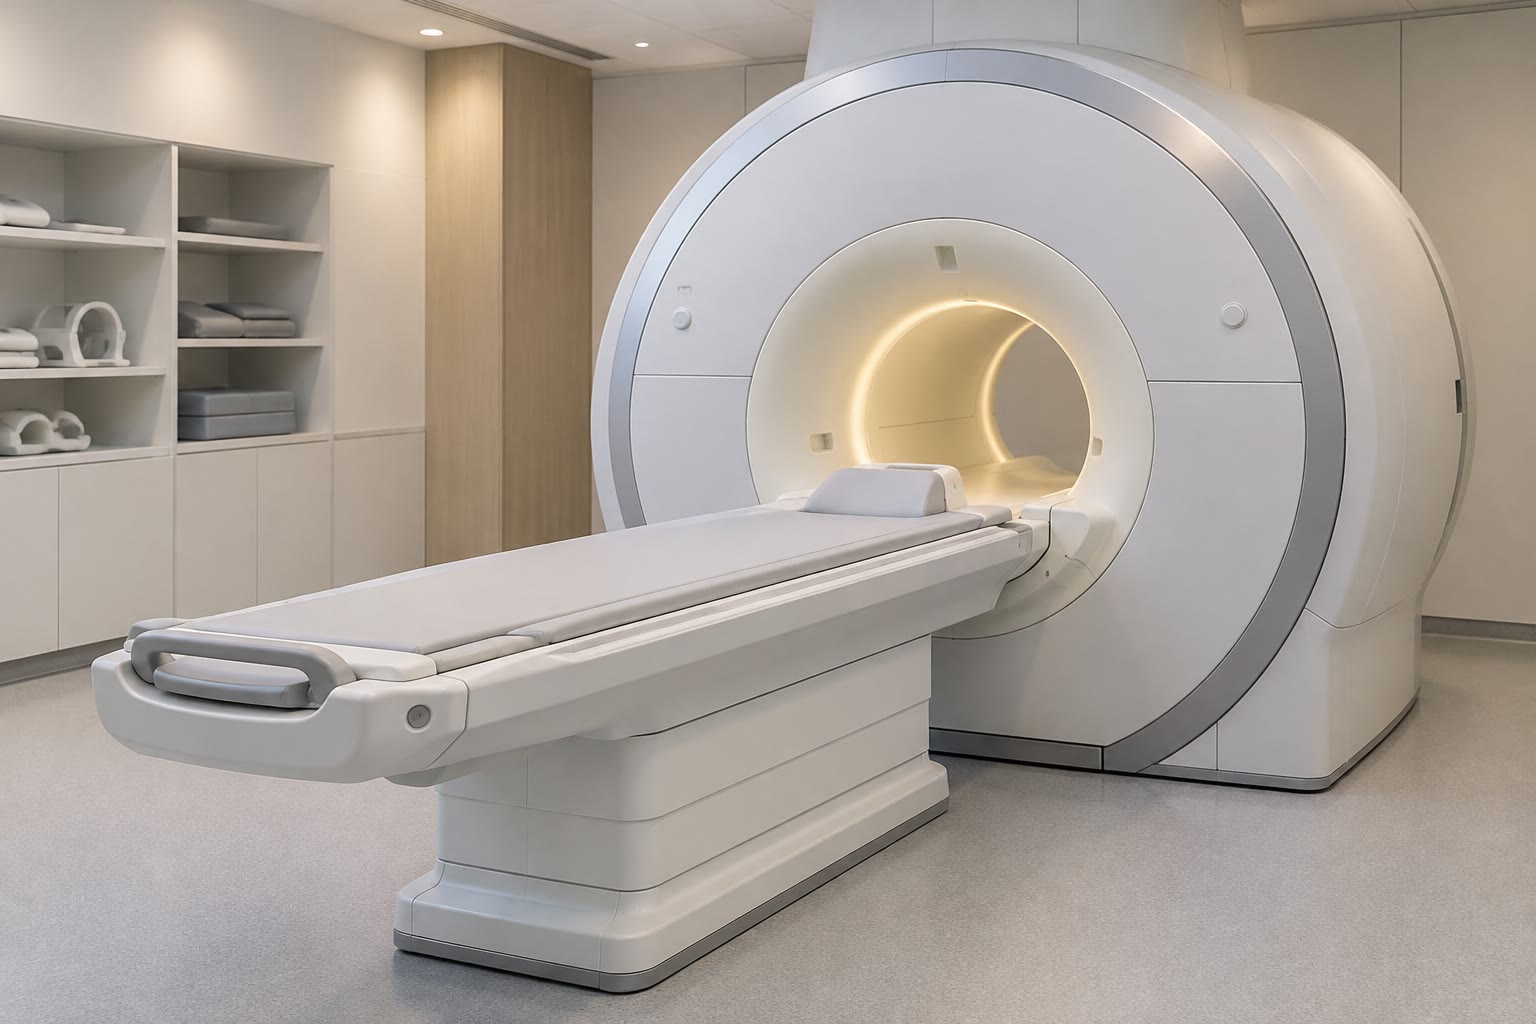
\includegraphics[width=0.48\linewidth]{images/book1/ai/g12-mri-room.jpg}

{\small Un appareil d'IRM~: la même physique que le spectromètre de RMN
du chimiste.}
\end{omfigure}

\section{Des protons dans un champ magnétique}

Le \omterm{def:g9:inside-the-atom:nucleus}{noyau} d'un \omterm{def:g7:atoms-and-molecules:atom}{atome} d'hydrogène est un simple \omterm{def:g9:inside-the-atom:proton}{proton}. Placé dans un champ
magnétique intense, il absorbe des ondes radio d'une fréquence précise~;
le comment et le pourquoi relèvent de la physique, et ne sont pas
nécessaires ici. Ce qui compte pour le chimiste, c'est que les \omterm{def:g9:inside-the-atom:nucleus}{électrons}
qui entourent un \omterm{def:g9:inside-the-atom:proton}{proton} l'écrantent légèrement du champ, et que cet
écrantage dépend des \omterm{def:g7:atoms-and-molecules:atom}{atomes} voisins~: un \omterm{def:g9:inside-the-atom:proton}{proton} proche d'un \omterm{def:g7:atoms-and-molecules:atom}{atome}
d'oxygène électronégatif, qui attire les \omterm{def:g9:inside-the-atom:nucleus}{électrons}, absorbe à une
fréquence légèrement différente de celle d'un \omterm{def:g9:inside-the-atom:proton}{proton} d'une chaîne
hydrocarbonée. Les différences sont infimes, quelques millionièmes de la
fréquence, et s'expriment en parties par million.

\begin{omfigure}
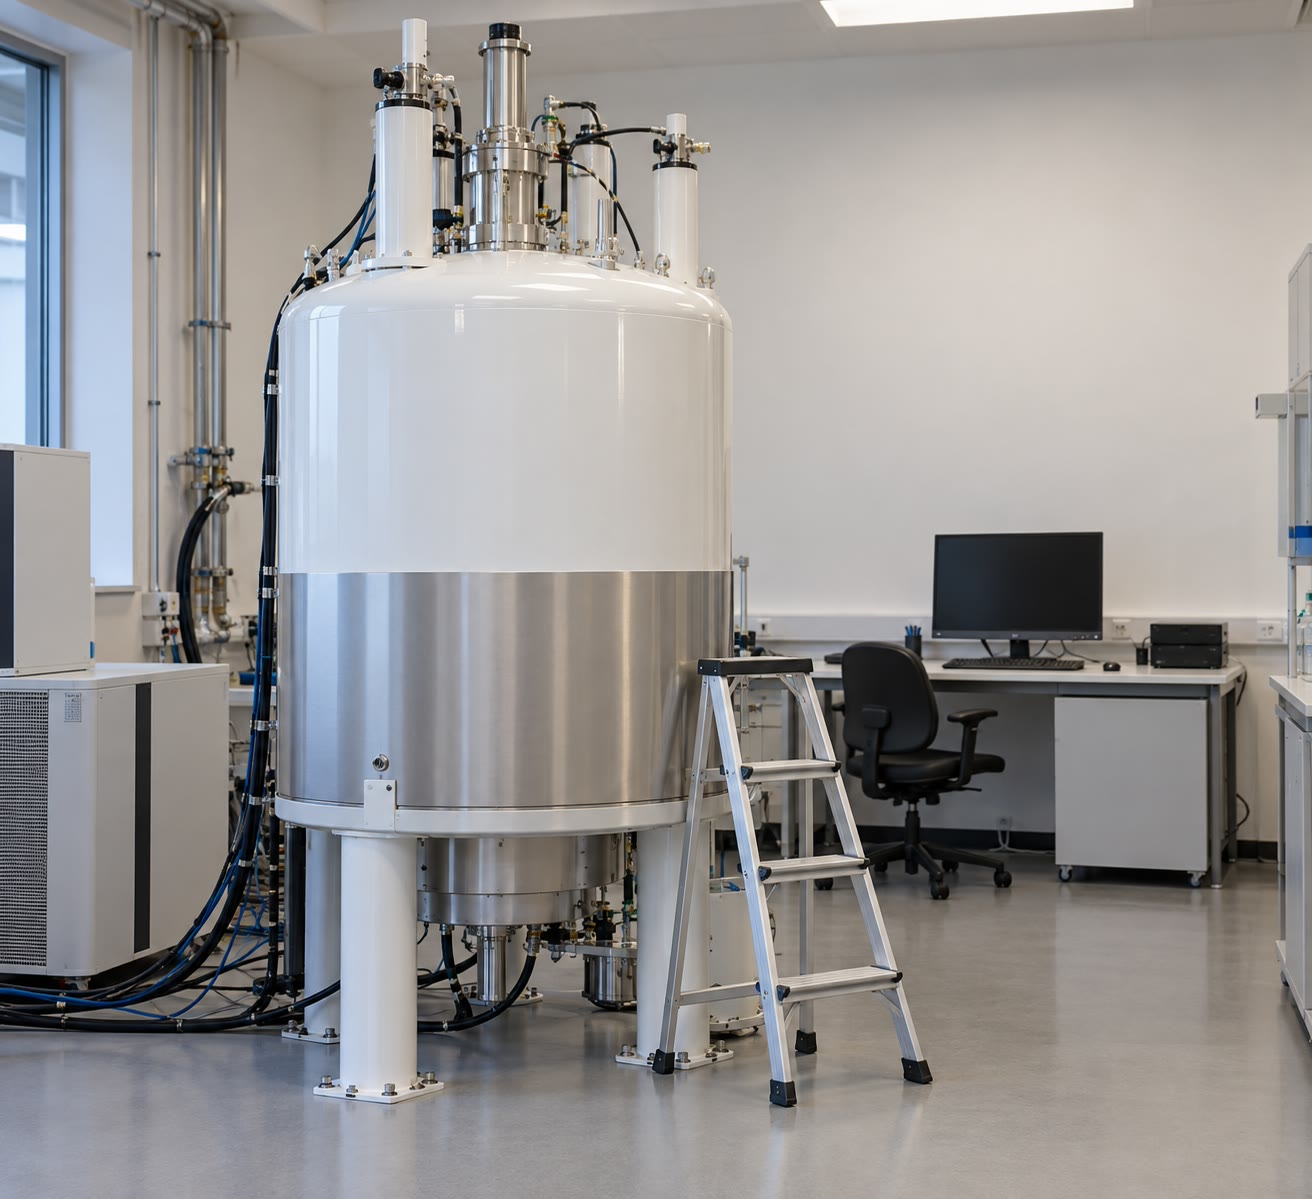
\includegraphics[width=0.42\linewidth]{images/book1/ai/g12-nmr-magnet.jpg}

{\small L'aimant d'un spectromètre de RMN.}
\end{omfigure}

\begin{definition}[Spectre de RMN, déplacement chimique]\label{def:g12:proton-nmr:spectrum}
Un \emph{spectre de RMN}\index{spectre de RMN} du \omterm{def:g9:inside-the-atom:proton}{proton} (résonance
magnétique nucléaire) montre les signaux absorbés par les noyaux
d'hydrogène d'un composé. La position d'un signal est son
\emph{déplacement chimique}\index{deplacement chimique@déplacement chimique} $\delta$, en
parties par million (\si{ppm}), mesuré à partir du signal d'un composé de
référence, le tétraméthylsilane \ce{Si(CH3)4} (TMS), placé à
$\delta = 0$. L'axe des $\delta$ est orienté de droite à gauche.
\end{definition}

\begin{proposition}[Le déplacement dépend des voisins]\label{prop:g12:proton-nmr:shift}
% ledger: nmrr:CH3, nmrr:CH2, nmrr:allylic, nmrr:ketone, nmrr:halide, nmrr:alcohol, nmrr:vinylic, nmrr:aryl, nmrr:aldehyde, nmrr:acid
Le \omterm{def:g12:proton-nmr:spectrum}{déplacement chimique} d'un \omterm{def:g9:inside-the-atom:proton}{proton} dépend des \omterm{def:g7:atoms-and-molecules:atom}{atomes} qui l'entourent~:
plus il est proche d'un \omterm{def:g7:atoms-and-molecules:atom}{atome} électronégatif ou d'une \omterm{def:g10:lewis-and-shape:multiple-bond}{double liaison},
plus son déplacement est grand. Domaines typiques, en \si{ppm}~:
\begin{center}
\small
\begin{tabular}{ll@{\qquad}ll}
\hline
environnement & $\delta$ & environnement & $\delta$ \\
\hline
\ce{CH3} d'une chaîne & 0.7--1.3 & \ce{H-C-O} (\omterm{def:g11:functional-groups:alcohol}{alcool}, éther, \omterm{def:g11:functional-groups:carboxylic-acid}{ester}) & 3.3--4.5 \\
\ce{CH2} d'une chaîne & 1.2--1.6 & \ce{H-C=C} & 4.5--6.5 \\
\ce{H-C-C=C} & 1.6--2.2 & H d'un cycle benzénique & 6.5--8.0 \\
\ce{H-C-C=O} & 2.0--2.4 & \omterm{def:g11:functional-groups:carbonyl}{aldéhyde} \ce{-CHO} & 9.7--10.0 \\
\ce{H-C-X} (\omterm{def:g10:electron-shells:family}{halogène}) & 2.5--4.0 & acide \ce{-COOH} & 11.0--12.0 \\
\hline
\end{tabular}
\end{center}
\end{proposition}

\begin{proof}
Valeurs mesurées sur de nombreux composés. Un voisin électronégatif
attire les \omterm{def:g9:inside-the-atom:nucleus}{électrons} loin du \omterm{def:g9:inside-the-atom:proton}{proton}, qui est moins écranté et absorbe à
un déplacement plus grand.
\end{proof}

\begin{omfigure}
\begin{tikzpicture}[font=\small, x=0.75cm, y=0.5cm]
  % delta axis reversed: x = 12 - delta
  \draw[->] (0,0) -- (12.4,0) node[right] {};
  \foreach \d in {12,11,10,9,8,7,6,5,4,3,2,1,0}
    \draw ({12-\d},0) -- ({12-\d},-0.2) node[below, font=\footnotesize] {\d};
  \node[below=14pt] at (6,-0.3) {$\delta$ (\si{ppm})};
  \foreach \a/\b/\y/\c/\l in {
      11.0/12.0/1/omThm/{\ce{COOH}},
      9.7/10.0/2/omThm/{\ce{CHO}},
      6.5/8.0/1/black!60/{cycle benzénique},
      4.5/6.5/2/omMeth/{\ce{C=C-H}},
      3.3/4.5/3/omDef/{\ce{H-C-O}},
      2.0/2.4/4/omProp/{\ce{H-C-C=O}},
      0.7/1.6/5/black!45/{\ce{CH3}, \ce{CH2} des chaînes}} {
    \fill[\c, rounded corners=1pt] ({12-\b},{\y-0.3}) rectangle ({12-\a},{\y+0.3});
    \node[anchor=west, font=\footnotesize] at ({12-\a+0.1},\y) {\l};
  }
  \draw[thick] (12,0) -- (12,0.6) node[above, font=\footnotesize] {TMS};
\end{tikzpicture}

{\small Où les \omterm{def:g9:inside-the-atom:proton}{protons} absorbent, selon leur environnement. Les \omterm{def:g9:inside-the-atom:proton}{protons}
proches d'un oxygène, d'une \omterm{def:g10:lewis-and-shape:multiple-bond}{double liaison} ou d'un groupe acide
apparaissent à gauche du spectre.}
\end{omfigure}

\begin{inthelab}[Préparer un tube de RMN]
On dissout quelques milligrammes du composé dans environ \qty{0.6}{mL}
d'un \omterm{def:g6:solutions-and-solubility:solute}{solvant} dont les \omterm{def:g7:atoms-and-molecules:atom}{atomes} d'hydrogène ont été remplacés par du
deutérium (\ce{CDCl3}, le chloroforme deutéré), qui ne donne aucun
signal~; on ajoute une trace de TMS comme référence. On filtre la
solution dans un tube de verre fin, que l'on bouche, étiquette et
descend dans l'aimant.
\end{inthelab}

\section{Les protons équivalents}

\begin{definition}[Protons équivalents]\label{def:g12:proton-nmr:equivalent}
Des \omterm{def:g9:inside-the-atom:proton}{protons} sont des \emph{protons équivalents}\index{protons equivalents@protons équivalents}
s'ils ont le même environnement dans la \omterm{def:g7:atoms-and-molecules:molecule}{molécule}, de sorte qu'ils
absorbent au même déplacement. Chaque groupe de \omterm{def:g9:inside-the-atom:proton}{protons} équivalents donne
un signal. Les trois \omterm{def:g9:inside-the-atom:proton}{protons} d'un groupe \ce{CH3} sont toujours
équivalents.
\end{definition}

\begin{example}[Compter les groupes]\label{ex:g12:proton-nmr:groups}
La propanone, \ce{CH3-CO-CH3}, a six \omterm{def:g9:inside-the-atom:proton}{protons} mais un seul groupe~: les
deux \ce{CH3} sont identiques, un de chaque côté du \ce{C=O}. L'éthanol,
\ce{CH3-CH2-OH}, a trois groupes (\ce{CH3}, \ce{CH2}, \ce{OH}), et
l'éthanoate d'éthyle, \ce{CH3-CO-O-CH2-CH3}, trois également~: le
\ce{CH3} voisin de \ce{C=O}, le \ce{CH2} voisin de \ce{O}, et le
\ce{CH3} en bout de chaîne.
\end{example}

\section{L'intégration}

\begin{definition}[Courbe d'intégration]\label{def:g12:proton-nmr:integration}
La \emph{courbe d'intégration}\index{courbe d'integration@courbe d'intégration} d'un \omterm{def:g12:proton-nmr:spectrum}{spectre
de RMN} est une courbe, tracée au-dessus des signaux, qui monte d'une
marche à chaque signal~: la hauteur de chaque marche est proportionnelle
au nombre de \omterm{def:g9:inside-the-atom:proton}{protons} qui donnent ce signal.
\end{definition}

\begin{example}[Lire les marches]\label{ex:g12:proton-nmr:steps}
Dans le spectre de l'éthanol, les marches au-dessus des trois signaux
mesurent 2, 1 et 3 unités, de gauche à droite~: \ce{CH2}, \ce{OH} et
\ce{CH3}. Seuls les rapports comptent~: des marches de 12, 6 et 18 mm
disent la même chose.
\end{example}

\section{La multiplicité et la règle des \texorpdfstring{$n+1$}{n+1}}


\begin{definition}[Multiplet, règle des $n+1$]\label{def:g12:proton-nmr:multiplet}
Un signal est souvent divisé en plusieurs raies proches~: c'est un
\emph{multiplet}\index{multiplet} (singulet, doublet, triplet,
quadruplet, \dots{} pour 1, 2, 3, 4 raies). Selon la
\emph{règle des $n+1$}\index{règle des n+1@règle des $n+1$}, un groupe de
\omterm{def:g12:proton-nmr:equivalent}{protons équivalents} dont les \omterm{def:g7:atoms-and-molecules:atom}{atomes} de carbone voisins portent $n$
\omterm{def:g9:inside-the-atom:proton}{protons} au total, non équivalents à lui, donne un signal de $n+1$ raies,
dont les intensités sont dans les rapports du triangle de Pascal.
\end{definition}

\begin{proposition}[Le couplage avec les voisins]\label{prop:g12:proton-nmr:n-plus-one}
Dans une \omterm{def:g7:atoms-and-molecules:molecule}{molécule} \ce{CH3-CH2-X} (X sans hydrogène), le signal du
\ce{CH3} est un triplet (2 \omterm{def:g9:inside-the-atom:proton}{protons} voisins) et celui du \ce{CH2} un
quadruplet (3 \omterm{def:g9:inside-the-atom:proton}{protons} voisins). Les \omterm{def:g9:inside-the-atom:proton}{protons} liés à un \omterm{def:g7:atoms-and-molecules:atom}{atome} d'oxygène ou
d'azote donnent en général un singulet et ne couplent pas avec leurs
voisins.
\end{proposition}

\begin{proof}
Admis~: chaque \omterm{def:g9:inside-the-atom:proton}{proton} voisin décale légèrement le signal vers le haut ou
vers le bas selon son propre état, et les combinaisons donnent $n+1$
raies~; la physique en est expliquée dans le volume de première année
d'université. Les \omterm{def:g9:inside-the-atom:proton}{protons} portés par O ou N s'échangent rapidement entre
\omterm{def:g7:atoms-and-molecules:molecule}{molécules}, ce qui moyenne leur effet.
\end{proof}

\begin{omfigure}
\begin{tikzpicture}[font=\small]
  % Pascal's triangle
  \foreach \r/\vals in {0/{1}, 1/{1,1}, 2/{1,2,1}, 3/{1,3,3,1}, 4/{1,4,6,4,1}} {
    \foreach \v [count=\i from 0] in \vals
      \node at ({\i*0.7 - \r*0.35}, {-\r*0.55}) {\v};
    \node[anchor=east, font=\footnotesize, black!60] at (-2.0,{-\r*0.55}) {$n = \r$};
  }
  % multiplets
  \begin{scope}[xshift=4.2cm, yshift=-2.4cm]
    \foreach \x/\name/\hs in {0/singulet/{1}, 1.4/doublet/{1,1}, 3.0/triplet/{1,2,1},
                              4.9/quadruplet/{1,3,3,1}} {
      \foreach \h [count=\i from 0] in \hs {
        \draw[very thick, omDef] ({\x + \i*0.22},0) -- ({\x + \i*0.22},{\h*0.55});
      }
      \node[anchor=north, font=\footnotesize] at ({\x+0.3},-0.1) {\name};
    }
  \end{scope}
\end{tikzpicture}

{\small Le triangle de Pascal donne les intensités relatives des $n+1$
raies d'un signal couplé à $n$ \omterm{def:g9:inside-the-atom:proton}{protons} voisins~: 1:1, 1:2:1, 1:3:3:1.}
\end{omfigure}

\begin{omfigure}
\newcommand{\nmrpanel}[4]{% file part, title, xmax, ymax
\begin{tikzpicture}
\begin{axis}[width=\linewidth, height=4.2cm, x dir=reverse, xmin=0,
    xmax=#3, ymin=0, ymax=#4, ytick=\empty, axis y line=none,
    axis x line*=bottom, xlabel={$\delta$ (\si{ppm})},
    tick label style={font=\scriptsize}, label style={font=\scriptsize},
    title={\small #2}, title style={yshift=-3pt}]
  \addplot[omDef, thin] table[x=delta, y=I] {figdata/out/grade-12-proton-nmr-#1.dat};
  \addplot[omProp, thick] table[x=delta, y expr=0.15+\thisrow{integral}*0.11]
    {figdata/out/grade-12-proton-nmr-#1.dat};
\end{axis}
\end{tikzpicture}}
\begin{minipage}{0.49\linewidth}\nmrpanel{a}{A~: éthanol}{5}{1.15}\end{minipage}\hfill
\begin{minipage}{0.49\linewidth}\nmrpanel{b}{B~: éthanoate d'éthyle}{5}{1.15}\end{minipage}

\begin{minipage}{0.49\linewidth}\nmrpanel{c}{C~: propanone}{5}{1.15}\end{minipage}\hfill
\begin{minipage}{0.49\linewidth}\nmrpanel{e}{D~: éthanoate de méthyle}{5}{1.15}\end{minipage}

\begin{minipage}{\linewidth}\nmrpanel{d}{E~: acide propanoïque}{12.5}{1.15}\end{minipage}

{\small \omterm{def:g12:proton-nmr:spectrum}{Spectres de RMN} du \omterm{def:g9:inside-the-atom:proton}{proton} (en bleu) avec leurs \omterm{def:g12:proton-nmr:integration}{courbes
d'intégration} (en orange~; chaque marche est proportionnelle au nombre
de \omterm{def:g9:inside-the-atom:proton}{protons} du signal situé en dessous). Les déplacements sont ceux de
spectres mesurés dans \ce{CDCl3}~; la forme et l'espacement des raies
sont tracés à partir d'un modèle simple.}
\end{omfigure}

\begin{example}[Lire les spectres]\label{ex:g12:proton-nmr:reading}
% ledger: nmr:ethylethanoate-OCH2, nmr:ethylethanoate-COCH3, nmr:ethylethanoate-CH3, nmr:ethanol-CH2, nmr:ethanol-CH3, nmr:ethanol-OH, nmr:acetone, nmr:propanoic-CH2, nmr:propanoic-CH3, nmr:propanoic-OH, nmr:meoac-OCH3, nmr:meoac-COCH3
L'éthanoate d'éthyle (B) donne un quadruplet de 2 \omterm{def:g9:inside-the-atom:proton}{protons} à
\qty{4.12}{ppm} (\ce{O-CH2}, voisin de l'oxygène et d'un \ce{CH3}), un
singulet de 3 \omterm{def:g9:inside-the-atom:proton}{protons} à
\qty{2.04}{ppm} (\ce{CH3-C=O}, sans \omterm{def:g9:inside-the-atom:proton}{proton} voisin) et un triplet de 3
\omterm{def:g9:inside-the-atom:proton}{protons} à \qty{1.26}{ppm} (\ce{CH3}, voisin d'un \ce{CH2}). La propanone
(C) donne un unique singulet de 6 \omterm{def:g9:inside-the-atom:proton}{protons} à \qty{2.16}{ppm}. L'acide
propanoïque (E) présente un quadruplet à \qty{2.39}{ppm}, un triplet à
\qty{1.16}{ppm}, et un singulet très à gauche, à \qty{11.7}{ppm}~: son
\omterm{def:g9:inside-the-atom:proton}{proton} acide.
\end{example}

\section{Utiliser ensemble l'infrarouge et la RMN}


\begin{method}[Identifier une molécule à partir de ses spectres IR et RMN]\label{met:g12:proton-nmr:identify}
\begin{enumerate}
  \item À partir de la \omterm{def:g11:organic-skeletons:formulas}{formule brute}, dresser la liste des \omterm{def:g11:organic-skeletons:isomer}{isomères}
        possibles et de leurs \omterm{def:g11:functional-groups:functional-group}{groupes caractéristiques}.
  \item Infrarouge~: chercher une bande \ce{C=O} vers \qty{1700}{cm^{-1}}
        et des bandes \ce{O-H} ou \ce{N-H}~; éliminer les \omterm{def:g11:organic-skeletons:isomer}{isomères} qui ne
        conviennent pas.
  \item RMN~: compter les signaux (groupes de \omterm{def:g12:proton-nmr:equivalent}{protons équivalents}), lire
        l'intégration (\omterm{def:g9:inside-the-atom:proton}{protons} par groupe), les multiplicités (voisins)
        et les déplacements (environnements).
  \item Assembler les éléments en une seule structure, et la confronter à
        chaque observation.
\end{enumerate}
\end{method}

\begin{example}[Deux isomères \ce{C3H6O2}]\label{ex:g12:proton-nmr:isomers}
L'acide propanoïque \ce{CH3-CH2-COOH} et l'éthanoate de méthyle
\ce{CH3-CO-O-CH3} sont \omterm{def:g11:organic-skeletons:isomer}{isomères}. En infrarouge, seul l'acide présente la
très large bande \ce{O-H}. En RMN (spectres E et D), l'acide donne un
triplet, un quadruplet et un singulet vers \qty{11.7}{ppm}~; l'\omterm{def:g11:functional-groups:carboxylic-acid}{ester}
donne deux singulets de 3 \omterm{def:g9:inside-the-atom:proton}{protons} chacun, à 3.66 (\ce{O-CH3}) et
\qty{2.05}{ppm} (\ce{CH3-C=O}), car aucun carbone de l'\omterm{def:g11:functional-groups:carboxylic-acid}{ester} ne porte de
\omterm{def:g9:inside-the-atom:proton}{protons} voisins d'un autre carbone porteur de \omterm{def:g9:inside-the-atom:proton}{protons}.
\end{example}

\section{Exercices}

\begin{exercise}[$\star$]\label{exo:g12:proton-nmr:1}
Combien de groupes de \omterm{def:g12:proton-nmr:equivalent}{protons équivalents}, et donc combien de signaux,
donnent ces \omterm{def:g7:atoms-and-molecules:molecule}{molécules}~: le méthane~; l'éthane \ce{CH3-CH3}~; le
propane~; le méthanol \ce{CH3-OH}~; le méthoxyméthane \ce{CH3-O-CH3}~?
\end{exercise}

\begin{exercise}[$\star$]\label{exo:g12:proton-nmr:2}
Un groupe de \omterm{def:g9:inside-the-atom:proton}{protons} a 2 \omterm{def:g9:inside-the-atom:proton}{protons} voisins sur le carbone adjacent.
Combien de raies son signal compte-t-il, et dans quels rapports~? Même
question pour 3 voisins et pour 0 voisin.
\end{exercise}

\begin{exercise}[$\star$]\label{exo:g12:proton-nmr:3}
Un spectre présente trois signaux dont les marches d'intégration mesurent
15, 10 et 15 mm. La \omterm{def:g7:atoms-and-molecules:molecule}{molécule} a 8 \omterm{def:g9:inside-the-atom:proton}{protons}. Combien de \omterm{def:g9:inside-the-atom:proton}{protons} chaque
signal représente-t-il~?
\end{exercise}

\begin{exercise}[$\star$]\label{exo:g12:proton-nmr:4}
À l'aide du tableau des déplacements, indiquer où l'on attend le signal
du \omterm{def:g9:inside-the-atom:proton}{proton} d'un groupe \omterm{def:g11:functional-groups:carbonyl}{aldéhyde}. Celui d'un groupe \ce{CH3} d'une
chaîne~?
\end{exercise}

\begin{exercise}[$\star$]\label{exo:g12:proton-nmr:5}
Pourquoi choisit-on comme référence le TMS, dont les \omterm{def:g9:inside-the-atom:proton}{protons} sont tous
équivalents~? Pourquoi le \omterm{def:g6:solutions-and-solubility:solute}{solvant} est-il deutéré~?
\end{exercise}

\begin{exercise}[$\star\star$]\label{exo:g12:proton-nmr:6}
Prévoir le spectre du chloroéthane \ce{CH3-CH2-Cl}~: nombre de signaux,
intégration, multiplicités, déplacements approximatifs.
\end{exercise}

\begin{exercise}[$\star\star$]\label{exo:g12:proton-nmr:7}
Prévoir le spectre du propan-2-ol, \ce{(CH3)2CH-OH}~: en particulier, la
multiplicité du signal des \ce{CH3} et de celui du \ce{CH} (on admet que
le \ce{OH} donne un singulet et ne couple pas).
\end{exercise}

\begin{exercise}[$\star\star$]\label{exo:g12:proton-nmr:8}
Trois spectres~: (a) un singulet~; (b) un quadruplet, un singulet et un
triplet, d'intégrations 2:3:3~; (c) un quadruplet, un triplet et un
singulet très à gauche, d'intégrations 2:3:1. Les associer à l'éthanoate
d'éthyle, à la propanone et à l'acide propanoïque.
\end{exercise}

\begin{exercise}[$\star\star$]\label{exo:g12:proton-nmr:9}
À l'aide du diagramme des déplacements, expliquer pourquoi le \ce{CH2}
de l'éthanoate d'éthyle (\qty{4.12}{ppm}) est situé loin à gauche du
\ce{CH3} du même groupe éthyle (\qty{1.26}{ppm}).
\end{exercise}

\begin{exercise}[$\star\star$]\label{exo:g12:proton-nmr:10}
Un composé \ce{C3H6O} présente une forte bande infrarouge à
\qty{1715}{cm^{-1}} et un unique singulet en RMN. L'identifier. Pourquoi
le propanal est-il exclu~?
\end{exercise}

\begin{exercise}[$\star\star$]\label{exo:g12:proton-nmr:11}
Dans le spectre de l'éthanol, pourquoi le signal du \ce{OH} est-il un
singulet, et pourquoi le \ce{CH2} apparaît-il comme un quadruplet plutôt
que comme un signal plus complexe~?
\end{exercise}

\begin{exercise}[$\star\star\star$]\label{exo:g12:proton-nmr:12}
Donner les structures de quatre \omterm{def:g11:organic-skeletons:isomer}{isomères} \ce{C4H8O2} qui sont des \omterm{def:g11:functional-groups:carboxylic-acid}{esters}
ou des acides (acide butanoïque, éthanoate d'éthyle, propanoate de
méthyle, méthanoate de propyle, \dots) et prévoir, pour chacun, le
nombre de signaux de RMN et leurs multiplicités.
\end{exercise}

\begin{exercise}[$\star\star\star$]\label{exo:g12:proton-nmr:13}
On agite une goutte d'eau lourde \ce{D2O} avec une solution d'éthanol,
et on enregistre de nouveau le spectre~: un signal disparaît. Lequel, et
pourquoi~? En quoi cela aide-t-il à reconnaître les \omterm{def:g9:inside-the-atom:proton}{protons} \ce{O-H}~?
\end{exercise}

\begin{exercise}[$\star\star\star$]\label{exo:g12:proton-nmr:14}
Un échantillon d'éthanoate d'éthyle contient un peu d'éthanol. Quels
signaux supplémentaires apparaissent dans le spectre~? Si l'intégration
du singulet à \qty{2.04}{ppm} mesure 30 mm et celle d'un petit triplet
supplémentaire à \qty{1.23}{ppm} mesure 3 mm, estimer le rapport des
quantités d'éthanol et d'\omterm{def:g11:functional-groups:carboxylic-acid}{ester}.
\end{exercise}

\begin{exercise}[$\star\star\star$]\label{exo:g12:proton-nmr:15}
Le 2-méthylpropan-1-ol a pour formule \ce{(CH3)2CH-CH2-OH}. Prévoir son
spectre~: les signaux, leurs intégrations, et la multiplicité des
signaux des \ce{CH3} et du \ce{CH2}. Quel signal compte le plus de
raies~?
\end{exercise}

\section{Problème~: le solvant inconnu}

\begin{problem}[{Problème du week-end --- un flacon de \omterm{def:g6:solutions-and-solubility:solute}{solvant} étiqueté
seulement \ce{C4H8O2}~: de quoi s'agit-il, et quelle est la hauteur de
chaque marche de sa \omterm{def:g12:proton-nmr:integration}{courbe d'intégration}~?}]
\label{pb:g12:proton-nmr:1}
% ledger: nmr:ethylethanoate-OCH2, nmr:ethylethanoate-COCH3, nmr:ethylethanoate-CH3, ir:CO-ester, ir:OH-acid
Un flacon de \omterm{def:g6:solutions-and-solubility:solute}{solvant}, dans une réserve, porte pour seule étiquette
«~\ce{C4H8O2}~». Son \omterm{def:g11:infrared:spectrum}{spectre infrarouge} présente une forte bande à
\qty{1740}{cm^{-1}} et aucune bande au-dessus de \qty{3100}{cm^{-1}}.
Son \omterm{def:g12:proton-nmr:spectrum}{spectre de RMN} présente trois signaux~: un quadruplet à
\qty{4.12}{ppm}, un singulet à \qty{2.04}{ppm} et un triplet à
\qty{1.26}{ppm}. La \omterm{def:g12:proton-nmr:integration}{courbe d'intégration} monte de \qty{72}{mm} au total.

\medskip
\noindent\textbf{Partie I --- Les candidats.}
\begin{enumerate}
  \item Vérifier que \ce{C4H8O2} convient à un \omterm{def:g11:functional-groups:carboxylic-acid}{ester} ou à un \omterm{def:g11:functional-groups:carboxylic-acid}{acide
        carboxylique} dont la chaîne ne comporte que des liaisons simples.
  \item Donner les \omterm{def:g11:organic-skeletons:formulas}{formules semi-développées} et les noms de l'acide
        butanoïque et des trois \omterm{def:g11:functional-groups:carboxylic-acid}{esters} éthanoate d'éthyle, propanoate de
        méthyle et méthanoate de propyle.
  \item Quel \omterm{def:g11:functional-groups:functional-group}{groupe caractéristique} ont-ils en commun deux à deux~?
\end{enumerate}

\medskip
\noindent\textbf{Partie II --- L'infrarouge.}
\begin{enumerate}[resume]
  \item Que révèle la bande à \qty{1740}{cm^{-1}}~?
  \item Que présenterait l'acide butanoïque qui manque ici~? L'éliminer.
  \item L'infrarouge seul permet-il de choisir entre les trois \omterm{def:g11:functional-groups:carboxylic-acid}{esters}~?
\end{enumerate}

\medskip
\noindent\textbf{Partie III --- La RMN.}
\begin{enumerate}[resume]
  \item Combien de groupes de \omterm{def:g12:proton-nmr:equivalent}{protons équivalents} l'inconnu a-t-il~?
  \item Que suggèrent ensemble le quadruplet et le triplet~?
  \item Que dit le singulet des voisins de ses \omterm{def:g9:inside-the-atom:proton}{protons}~?
  \item Pourquoi le quadruplet est-il à un grand déplacement~?
  \item Prévoir le spectre du propanoate de méthyle
        \ce{CH3-CH2-CO-O-CH3} (signaux, multiplicités, déplacements
        approximatifs). Est-ce l'inconnu~?
  \item Prévoir le spectre du méthanoate de propyle. Est-ce l'inconnu~?
\end{enumerate}

\medskip
\noindent\textbf{Partie IV --- Identification et intégration.}
\begin{enumerate}[resume]
  \item Identifier l'inconnu et dessiner sa structure, en attribuant
        chaque signal.
  \item Combien de \omterm{def:g9:inside-the-atom:proton}{protons} chaque signal représente-t-il~?
  \item L'intégration totale est de \qty{72}{mm} pour 8 \omterm{def:g9:inside-the-atom:proton}{protons}. Combien
        de millimètres par \omterm{def:g9:inside-the-atom:proton}{proton}~?
  \item Calculer la hauteur de la marche du singulet et de celle du
        triplet.
  \item Vérifier que les trois marches totalisent \qty{72}{mm}.
  \item L'éthanoate d'éthyle sent le bonbon anglais~: est-ce cohérent
        avec la famille trouvée~?
  \item Donner la réponse finale~: quelle est la hauteur de la marche
        d'intégration du quadruplet~?
\end{enumerate}
\end{problem}
